\documentclass{thomasClass}

\title{\textbf{Required Practical 3}
\\Production of a dilution series of a solute to produce a calibration curve with which to identify the water potential of plant tissue\\
{\Large Attempt 2 - Bell Peppers}
}
\author{Thomas Boxall}
\date{March 2022}
\begin{document}

\maketitle

\section{Apparatus}
\begin{itemize}
    \item Quarter of a bell pepper;
    \item $50cm^3$ 1M sucrose solution;
    \item $75cm^3$ distilled water;
    \item 11 test tubes;
    \item 2 $10cm^3$ graduated pipettes;
    \item 2 pipette fillers;
    \item Cutting tile;
    \item Scalpel;
    \item Petri dish with lid;
    \item Paper towels.
\end{itemize}

\section{Method}
\begin{enumerate}
    \item Use a permanent marker to label 11 test tubes with each molarity in the dilution series.
    \item Using the table below and one graduated pipette and one pipette filler for each of the sucrose solution \& distilled water, prepare the dilution series.
    \begin{table}[H]
    \centering
    \begin{tabularx}{0.8\textwidth}{XXX}
    Molarity of Sucrose Solution/M & Volume of distilled water ($CM^3$) & Volume of 1M sucrose solution ($CM^3$) \\
    \hline
    0.0 & 5.0 & 0.0 \\
    0.1 & 4.5 & 0.5 \\
    0.2 & 4.0 & 1.0 \\
    0.3 & 3.5 & 1.5 \\
    0.4 & 3.0 & 2.0 \\
    0.5 & 2.5 & 2.5 \\
    0.6 & 2.0 & 3.0 \\
    0.7 & 1.5 & 3.5 \\
    0.8 & 1.0 & 4.0 \\
    0.9 & 0.5 & 4.5 \\
    1.0 & 0.0 & 5.0
    \end{tabularx}
    \caption{Concentration calibration values}
    \label{tab:conCal}
    \end{table}
    
    \item Get the pepper out and orientate it on the cutting tile so that the giant cells are running from the top of the pepper to the bottom of the pepper.
    \item Avoiding sections of pericarp with white pith, use the scalpel to cut a strip into pieces 1cm long and 0.5cm wide.
    \item Places the pieces into a petri dish and cover with a lid until ready to record their masses.
    \item Quickly rinse the pieces in distilled water and gently-yet-thoroughly pat dry with a paper towel, just before weighing.
    \item Once a piece of pepper has been weighed and its mass recorded in a results table, place it into the correct tube of sucrose solution and leave for 30 minutes.
    \item After 30 minutes, remove the pieces of pepper from the sucrose solution, pat dry and re-weigh.
    \item Record the data in a data table.
    \item For each tube, calculate percentage change in mass of the tissue.\\
    $\displaystyle \mathrm{Percentage\ Change\ In\ Mass} = \frac{\mathrm{Change\ In\ Mass}}{\mathrm{Original\ Mass}} \times 100$
    \item Plot a graph to show this data. Use the concentration of the solution on the $x$ axis and the change in mass along the $y$ axis.
\end{enumerate}

\section{Safety \& Risk Assessment}
\begin{itemize}
    \item Avoid contact with the pepper tissue if you are allergic to it. If you come into contact with it and suffer an allergic reaction, rinse the affected area thoroughly under cold running water. Seek further medical attention if necessary.
    \item Take care when using sharp instruments. When they are not in use, replace covers or place then on the bench.
    \item The neck of the graduated pipette is fragile and could easily snap when attaching or removing the pipette filler, take care not to snap it.
\end{itemize}

\section{Results}
\begin{table}[H]
\centering
\begin{tabularx}{1\textwidth}{X|X|X|X|X}
Sucrose Concentration (M) & Pepper Mass Before (g) & Pepper Mass After (g) & Change In Mass (g) & Percentage Change In Mass (\%) \\
\hline
0 & 0.38 & 0.41 & 0.03 & 0.07894736842 \\
0.1 & 0.31 & 0.33 & 0.02 & 0.06451612903 \\
0.2 & 0.33 & 0.35 & 0.02 & 0.06060606061 \\
0.3 & 0.36 & 0.38 & 0.02 & 0.05555555556 \\
0.4 & 0.33 & 0.34 & 0.01 & 0.0303030303 \\
0.5 & 0.36 & 0.37 & 0.01 & 0.02777777778 \\
0.6 & 0.35 & 0.36 & 0.01 & 0.02857142857 \\
0.7 & 0.37 & 0.37 & 0 & 0 \\
0.8 & 0.27 & 0.26 & -0.01 & -0.03703703704 \\
0.9 & 0.41 & 0.41 & 0 & 0 \\
1 & 0.39 & 0.39 & 0 & 0
\end{tabularx}
\caption{Data from experiment}
\label{tab:data}
\end{table}
\begin{figure}[H]
    \centering
    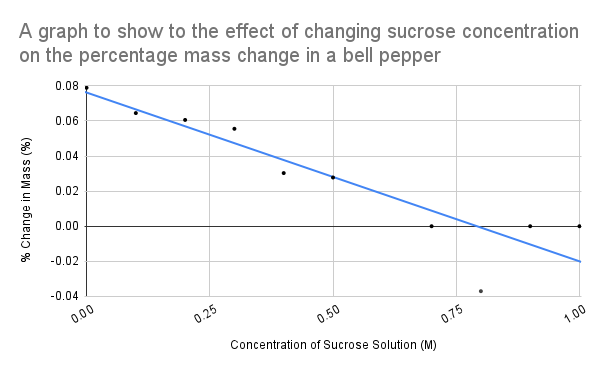
\includegraphics[width=0.8\textwidth]{graph.png}
    \caption{Graph produced using Google Sheets}
    \label{fig:graph}
\end{figure}


\section{Evaluation Questions}
\begin{enumerate}
    \item \textbf{Why are the pepper pieces stored in a covered dish until they are needed?}\\
    To prevent them drying out from being exposed to the air which would change their water content therefore change their water potential.
    \item \textbf{Why are the discs washed in distilled water?}\\
    To make sure that they don't have any fluids on them which have escaped from cells when they were cut. These fluids may contain starch molecules or glucose which would skew the results. 
    \item \textbf{Why are they dried very carefully?}\\
    They are dried very carefully to remove any surface water which would potentially skew the results.
    \item \textbf{Explain why the pieces of pepper are left in the solution for 30 minutes. After 30 minutes what happens to the next diffusion of water molecules?}\\
    The peppers are left in the solutions for 30 minutes to allow the pepper piece and solution to reach dynamic equilibrium. This will be when net movement of particles stops. 
    \item \textbf{Why was change in mass data converted into percentage change in the mass in this investigation?}\\
    So that any differences in the masses of the pepper pieces weren't carried through to the final results of the experiment. All the pepper pieces should have been the same mass.
    \item \textbf{Use your graph to find which molarity of sucrose solution has the same water potential as the pepper. Explain how you got your answer.}\\
    0.8M. I reached this answer by looking at where the line of best fit on my graph crossed the X axis. 
    \item \textbf{Explain fully the shape of the graph in terms of water potential (i.e. why some pieces of pepper gain mass, why some loose mass and why some may stay the same). In your answer use the following terms: Osmosis, water potential, water potential gradient, net movement of water molecules.}\\
    Some pieces of pepper gain mass. These are the pieces of pepper which are placed in the lowest molarity solution, which will have the least negative water potential therefore there is a net movement of water molecules into the pepper therefore it will gain mass, this will be down a water potential gradient. At the other end of the scale, the more concentrated solutions will draw the water out of the pepper therefore it will loose mass. This is due to osmosis.  
    \item \textbf{What is your estimate of the water potential of the pepper pericarp tissue cells?}\\
    -2.61MPa
    \item \textbf{Explain how you obtained a value for the water potential of the cells in the pepper pericarp tissue.}\\
    Using my graph, I looked at where the line of best fit intercepts the $x$ axis. This is at around 0.8M, I then used a reference table\footnote{http://www.saps.org.uk/attachments/article/286/SAPS\%20Water\%20Potential\%20of\%20a\%20Potato\%20Cell\%20-\%20student\%20notes.doc} to get the corresponding water potential. 
    \item \textbf{How could you increase the reliability of this investigation?}\\
    To increase the reliability of this investigation, I would need to repeat it multiple times with similar bell peppers and use a mean of all of my percentage change in mass results.
    \item \textbf{Compare the value for water potential of pericarp cells that you obtained with that obtained by other students in your class, using different pieces of capsicum pericarp tissue. Discuss the possible causes of similarities and differences within the class.}\\
    Another person in my class got -1.82MPa for their water potential. This was using the same pepper. This could have been because of a difference in the concentration due to error, a difference in the time which it was allowed to soak for or a difference in the pepper depending on what side it came from.  
    
\end{enumerate}


\end{document}
